
\chapter{洞察}
\label{chap:insight}

{\bfseries\large 这里的内容,很多都是错误有误导的,如果你是容易被人误导的人,那么建议你不要继续看本节的内容,不要看,不要看,千万不要看。}\clearpage\pagebreak

\section{错误的证明}
\label{sec:wrong-proof}


\begin{example}[消失的方块]证明:$31.5=32.5$。

  \centering
  \begin{tikzpicture}[scale=0.6,line join=round]
    \begin{scope}[shift={(0,0)}]
      \draw[very thick,pattern=north east lines, pattern color=black](1,1)--(9,1)--(9,4)--cycle;
      \draw[very thick,pattern=dots, pattern color=red](9,1)--(14,1)--(14,3)--(11,3)--(11,2)--(9,2)--cycle;
      \draw[very thick,pattern=bricks, pattern color=blue](14,3)--(11,3)--(11,2)--(9,2)--(9,4)--(14,4)--cycle;
      \draw[very thick,pattern=checkerboard, pattern color=violet](9,4)--(14,4)--(14,6)--cycle;
      % \draw[very thick](1,1)--(14,1)--(14,6)--(9,4)--cycle;
      \draw[help lines](0,0)grid(15,7);
    \end{scope}
    \begin{scope}[shift={(0,-8)}]
      \draw[very thick,xshift=5cm,yshift=2cm,pattern=north east lines, pattern color=black](1,1)--(9,1)--(9,4)--cycle;
      \draw[very thick,pattern=dots, pattern color=red](9,1)--(14,1)--(14,3)--(11,3)--(11,2)--(9,2)--cycle;
      \draw[very thick,xshift=-3cm,yshift=-1cm,pattern=bricks, pattern color=blue](14,3)--(11,3)--(11,2)--(9,2)--(9,4)--(14,4)--cycle;
      \draw[very thick,xshift=-8cm,yshift=-3cm,pattern=checkerboard, pattern color=violet](9,4)--(14,4)--(14,6)--cycle;
      \draw[help lines](0,0)grid(15,7);
      % \draw[very thick](1,1)--(14,1)--(14,6)--(6,3)--cycle;
    \end{scope}
    \begin{scope}[shift={(0,-16)}]
      % \draw[very thick,xshift=5cm,yshift=2cm,pattern=north east lines, pattern color=black](1,1)--(9,1)--(9,4)--cycle;
      % \draw[very thick,pattern=dots, pattern color=red](9,1)--(14,1)--(14,3)--(11,3)--(11,2)--(9,2)--cycle;
      % \draw[very thick,xshift=-3cm,yshift=-1cm,pattern=bricks, pattern color=blue](14,3)--(11,3)--(11,2)--(9,2)--(9,4)--(14,4)--cycle;
      % \draw[very thick,xshift=-8cm,yshift=-3cm,pattern=checkerboard, pattern color=violet](9,4)--(14,4)--(14,6)--cycle;
      \draw[help lines](0,0)grid(15,7);
      \draw(1,1)--(6,3)--(14,6)--(9,4)--cycle;
      %\draw(1,1)--(14,6);
      %\draw[very thick](1,1)--(14,1)--(14,6)--(6,3)--cycle;
      \foreach \x/\y in {1/1,6/3,9/4,14/6}{%
        \draw(\x,\y)circle(2pt);
      }
    \end{scope}
  \end{tikzpicture}
\end{example}

\begin{proof}
  考虑阴影部分总面积,由上图,其面积为$\dfrac12\times13\times5=32.5$;由下图,其面积为$32.5-1=31.5$。而上下两图都是由相同组件组成,其面积应相同,从而有$32.5=31.5$。

  然而结论显然是错误的,也就是证明也是错误的。注意最后一图中四个点并不在一条直线上,所以根本原因在于最大的“三角形”并不是真正的三角形。差出来的一个格子的面积,就是图中四个点组成的四边形的面积\footnote{如果看不清的话,在电子文档上放大看。}。
\end{proof}


\fbox{\bfseries\noindent
  \begin{minipage}{.9\linewidth}
    注意!以下大多数的的求和“方法”在通常定义下都是错误的,请注意分辩。
  \end{minipage}
}

\begin{definition}[交错级数,Alternating Series]
  若$a_n\ge 0$,则$\sum(-1)^n a_n$称为交错级数,即正负相间的级数。
\end{definition}

\begin{theorem}[莱布尼茨定理]
  若交错级数中各项非负数列单调且趋于0,则级数收敛。即$\forall n$,$a_n\ge0$且$a_n\ge a_{n+1}$,则$\sum (-1)^n a_n$收敛,且其和$s\le a_1$(设$a_1$是第一个非0项),其余项$r_n$满足$|r_n|\le a_{n+1}$。
\end{theorem}
\begin{proof}[提示]
  $S_{n+1}-S_n=(-1)^{n+1} a_{n+1}$,从而$|S_n| - a_{n+1} \le |S_{n+1}|\le |S_n| + a_{n+1}$。
\end{proof}

\begin{definition}[阿贝尔和]
  $A(s)\equiv\lim\limits_{z\to1^{-}}\sum\limits_{n=1}^\infty a_nz^n$称为数列$s=\{a_1,a_2,\cdots\}$的阿贝尔和。
\end{definition}
\begin{example}[交错级数,Alternating Series]
  $1-2+3-4+5-6+\cdots$的阿贝尔和为$\frac14$。

  欧拉也曾研究过这个级数,他的设想与阿贝尔求和相似,他应用了如下的等式:
  \begin{align*}
    \frac1{(1+x)^2} = 1 - 2x + 3x^2 - 4x^3 + \cdots 
  \end{align*}
  至少这个等式在$|x|<1$时是成立,有很多种证明方法,比如泰勒展开,比如多项式长除。从而令$x$从左侧趋向于1,则可得级数的阿贝尔和为$\lim\limits_{x\to1^-}\dfrac{1}{(1+x)^2}=\frac14$。

  %\fbox{\noindent\begin{minipage}{.9\textwidth}
      也可以用一种直观的移位方式求出此交错级数的和。令
      \begin{align*}
        S_0 = 1 - 2 + 3 - 4 + \cdots
      \end{align*}
      将4个$S_0$相加,移位,上下对应位置数字相加,可得
      \begin{align*}\setlength\arraycolsep{2pt}
        \begin{array}{rccccccccccccc}
          4S_0 = &   &  &  &  &  &1 & -&2 & +&3 & -&4 & \cdots\\
                 & + &  &  &1  & -&2 & +&3 & -&4 & +&5 & \cdots\\
                 & + &  &  &1  & -&2 & +&3 & -&4 & +&5 & \cdots\\
                 & + &1 & -&2 & +&3 & -&4 & +&5 & -&6 & \cdots\\
               = &   &1 & +&0 & +&0 & +&0 & +&0 & +&0 & \cdots\\
               = &   &1
        \end{array}
      \end{align*}
      从而有$S_0=\frac14$。按这种方式,也可以得到$1-1+1-1+1-1+\cdots=\frac12$。问题出在哪里呢?如果序列是有限的,方法也许是可行的,然而对于无限的序列,特别是和是发散的无限级数,其和的定义都是不明确的,得出的结论自然也就与常识不符合。
    %\end{minipage}
  %}
\end{example}


\begin{example}
  所有正整数的和是$-\frac1{12}$。

  虽然这是个明显错误的结论,但下面的“证明”却“表明”了它是正确的,你能想明白为什么吗?

  \fbox{\small\begin{minipage}{.9\textwidth}
    令
    \begin{align*}
      S\phantom{_0}   =1+2+3+4+5+6+\cdots\\
      S_0 =1-2+3-4+5-6+\cdots
    \end{align*}
    那么
    \begin{align*}
      S - S_0 = 0 + 4 + 0 + 8 + 0 + 12 + 0 + \cdots = 4S
    \end{align*}
    从而$3S=-S_0$,由上面的交错级数和例子,有$S=-\frac1{12}$。
  \end{minipage}}
\end{example}

\section{数数}
\label{sec:count}


\begin{example}数一数,下面的图中有多少个三角形?
  \begin{center}
    \begin{tikzpicture}[scale=1.0]
      \coordinate(A) at (0,0);
      \coordinate(B) at (1,0);
      \coordinate(C) at (2,0);
      \coordinate(D) at (3,0);
      \coordinate(F) at (1.5,2);
      \coordinate(E) at ($.5*(D)+.5*(F)$);
      \coordinate(G) at ($.75*(B)+.25*(F)$);
      \coordinate(H) at ($.6*(C)+.4*(F)$);
      \draw(A)--(D)--(F)--(A)--(G)--(H)--(E) (B)--(F)--(C);
    \end{tikzpicture}
  \end{center}
\end{example}
\begin{proof}[提示]
  单个格子组成的三角形:
  \begin{center}
    \begin{tikzpicture}[scale=.75]
      \foreach \dx/\dy/\VA/\VB/\VC in {%
        0/0/A/B/G,
        4/0/A/F/G,
        8/0/F/G/H,
        12/0/F/H/E}{%
          \begin{scope}[shift={(\dx,\dy)}]
            \coordinate(A) at (0,0);
            \coordinate(B) at (1,0);
            \coordinate(C) at (2,0);
            \coordinate(D) at (3,0);
            \coordinate(F) at (1.5,2);
            \coordinate(E) at ($.5*(D)+.5*(F)$);
            \coordinate(G) at ($.75*(B)+.25*(F)$);
            \coordinate(H) at ($.6*(C)+.4*(F)$);
            \fill[color=red!20](\VA)--(\VB)--(\VC)--cycle;
            \draw(A)--(D)--(F)--(A)--(G)--(H)--(E) (B)--(F)--(C);
          \end{scope}
        }
    \end{tikzpicture}
  \end{center}

  两个格子组成的三角形:
  \begin{center}
    \begin{tikzpicture}[scale=.75]
      \foreach \dx/\dy/\VA/\VB/\VC in {%
        0/0/A/B/F,
        4/0/B/C/F,
        8/0/C/D/F,
        0/-3/A/C/H,
        4/-3/A/H/F,
        8/-3/G/E/F}{%
          \begin{scope}[shift={(\dx,\dy)}]
            \coordinate(A) at (0,0);
            \coordinate(B) at (1,0);
            \coordinate(C) at (2,0);
            \coordinate(D) at (3,0);
            \coordinate(F) at (1.5,2);
            \coordinate(E) at ($.5*(D)+.5*(F)$);
            \coordinate(G) at ($.75*(B)+.25*(F)$);
            \coordinate(H) at ($.6*(C)+.4*(F)$);
            \fill[color=red!20](\VA)--(\VB)--(\VC)--cycle;
            \draw(A)--(D)--(F)--(A)--(G)--(H)--(E) (B)--(F)--(C);
          \end{scope}
        }
    \end{tikzpicture}
  \end{center}

  其余3个格子、4个格子、5个格子和6个格子组成的三角形请自行考虑。
\end{proof}
\begin{proof}[另外一种数法]
  将所有的小格子排序,数出包含第一个格子所有的三角形。然后将图形挖掉第一个格子后,再数出包含第二个格子的所有的三角形。然后再继续挖掉第二个小格子,再数出包含第三个小格子的所有的三角形。依次下去可得。

  首先对小格子编号。
    \begin{center}
    \begin{tikzpicture}[scale=.75]
      \begin{scope}[shift={(0,0)}]
        \coordinate(A) at (0,0);
        \coordinate(B) at (1,0);
        \coordinate(C) at (2,0);
        \coordinate(D) at (3,0);
        \coordinate(F) at (1.5,2);
        \coordinate(E) at ($.5*(D)+.5*(F)$);
        \coordinate(G) at ($.75*(B)+.25*(F)$);
        \coordinate(H) at ($.6*(C)+.4*(F)$);
        \draw(A)--(D)--(F)--(A)--(G)--(H)--(E) (B)--(F)--(C);
        \foreach \x/\y/\z/\v in {A/B/G/1,A/G/F/4,H/G/F/5,H/E/F/6}{%
          \node at($1/3*(\x)+1/3*(\y)+1/3*(\z)$){\tiny \v};
        }
        \foreach \x/\y/\z/\w/\v in {B/C/G/H/2,C/D/E/H/3}{%
          \node at($1/4*(\x)+1/4*(\y)+1/4*(\z)+1/4*(\w)$){\tiny \v};
        }
      \end{scope}
    \end{tikzpicture}
  \end{center}
  数出含格子1的三角形。
  \begin{center}
    \begin{tikzpicture}[scale=.75]
      \foreach \dx/\dy/\VA/\VB/\VC in {%
        0/0/A/B/G,
        4/0/A/C/H,
        8/0/A/D/E,
        0/-3/A/B/F,
        4/-3/A/C/F,
        8/-3/A/D/F}{%
          \begin{scope}[shift={(\dx,\dy)}]
            \coordinate(A) at (0,0);
            \coordinate(B) at (1,0);
            \coordinate(C) at (2,0);
            \coordinate(D) at (3,0);
            \coordinate(F) at (1.5,2);
            \coordinate(E) at ($.5*(D)+.5*(F)$);
            \coordinate(G) at ($.75*(B)+.25*(F)$);
            \coordinate(H) at ($.6*(C)+.4*(F)$);
            \fill[color=red!20](\VA)--(\VB)--(\VC)--cycle;
            \draw(A)--(D)--(F)--(A)--(G)--(H)--(E) (B)--(F)--(C);
            \node at($1/3*(A)+1/3*(B)+1/3*(G)$){\tiny 1};
          \end{scope}
        }
    \end{tikzpicture}
  \end{center}
  挖掉格子1,找出所有包含格子2的三角形,有2个。
    \begin{center}
    \begin{tikzpicture}[scale=.75]
      \foreach \dx/\dy/\VA/\VB/\VC in {%
        0/0/B/B/B,
        4/0/B/C/F,
        8/0/B/D/F}{%
          \begin{scope}[shift={(\dx,\dy)}]
            \coordinate(A) at (0,0);
            \coordinate(B) at (1,0);
            \coordinate(C) at (2,0);
            \coordinate(D) at (3,0);
            \coordinate(F) at (1.5,2);
            \coordinate(E) at ($.5*(D)+.5*(F)$);
            \coordinate(G) at ($.75*(B)+.25*(F)$);
            \coordinate(H) at ($.6*(C)+.4*(F)$);
            \fill[color=red!20](\VA)--(\VB)--(\VC)--cycle;
            \draw(B)--(D)--(F)--cycle (E)--(A)--(F)--(C);
            \foreach \x/\y/\z/\v in {A/G/F/4,H/G/F/5,H/E/F/6}{%
              \node at($1/3*(\x)+1/3*(\y)+1/3*(\z)$){\tiny \v};
            }
            \foreach \x/\y/\z/\w/\v in {B/C/G/H/2,C/D/E/H/3}{%
              \node at($1/4*(\x)+1/4*(\y)+1/4*(\z)+1/4*(\w)$){\tiny \v};
            }
          \end{scope}
        }
    \end{tikzpicture}
  \end{center}
  继续挖掉格子2,找出所有包含格子3的三角形,也只有1个。
    \begin{center}
    \begin{tikzpicture}[scale=.75]
      \foreach \dx/\dy/\VA/\VB/\VC in {%
        0/0/C/C/C,
        4/0/D/C/F}{%
          \begin{scope}[shift={(\dx,\dy)}]
            \coordinate(A) at (0,0);
            \coordinate(B) at (1,0);
            \coordinate(C) at (2,0);
            \coordinate(D) at (3,0);
            \coordinate(F) at (1.5,2);
            \coordinate(E) at ($.5*(D)+.5*(F)$);
            \coordinate(G) at ($.75*(B)+.25*(F)$);
            \coordinate(H) at ($.6*(C)+.4*(F)$);
            \fill[color=red!20](\VA)--(\VB)--(\VC)--cycle;
            \draw(E)--(A)--(F)--(D)--(C)--(F)--(G);
            \foreach \x/\y/\z/\v in {A/G/F/4,H/G/F/5,H/E/F/6}{%
              \node at($1/3*(\x)+1/3*(\y)+1/3*(\z)$){\tiny \v};
            }
            \foreach \x/\y/\z/\w/\v in {C/D/E/H/3}{%
              \node at($1/4*(\x)+1/4*(\y)+1/4*(\z)+1/4*(\w)$){\tiny \v};
            }
          \end{scope}
        }
    \end{tikzpicture}
  \end{center}
  继续挖掉格子3,找出所有包含格子4的三角形。
    \begin{center}
    \begin{tikzpicture}[scale=.75]
      \foreach \dx/\dy/\VA/\VB/\VC in {%
        0/0/A/A/A,
        4/0/A/G/F,
        8/0/A/H/F,
        12/0/A/E/F}{%
          \begin{scope}[shift={(\dx,\dy)}]
            \coordinate(A) at (0,0);
            \coordinate(B) at (1,0);
            \coordinate(C) at (2,0);
            \coordinate(D) at (3,0);
            \coordinate(F) at (1.5,2);
            \coordinate(E) at ($.5*(D)+.5*(F)$);
            \coordinate(G) at ($.75*(B)+.25*(F)$);
            \coordinate(H) at ($.6*(C)+.4*(F)$);
            \fill[color=red!20](\VA)--(\VB)--(\VC)--cycle;
            \draw(G)--(F)--(E)--(A)--(F)--(H);
            \foreach \x/\y/\z/\v in {A/G/F/4,H/G/F/5,H/E/F/6}{%
              \node at($1/3*(\x)+1/3*(\y)+1/3*(\z)$){\tiny \v};
            }
          \end{scope}
        }
    \end{tikzpicture}
  \end{center}
  继续挖掉格子4,找出所有包含格子5的三角形,有2个。
    \begin{center}
    \begin{tikzpicture}[scale=.75]
      \foreach \dx/\dy/\VA/\VB/\VC in {%
        0/0/F/F/F,
        4/0/H/G/F,
        8/0/E/G/F}{%
          \begin{scope}[shift={(\dx,\dy)}]
            \coordinate(A) at (0,0);
            \coordinate(B) at (1,0);
            \coordinate(C) at (2,0);
            \coordinate(D) at (3,0);
            \coordinate(F) at (1.5,2);
            \coordinate(E) at ($.5*(D)+.5*(F)$);
            \coordinate(G) at ($.75*(B)+.25*(F)$);
            \coordinate(H) at ($.6*(C)+.4*(F)$);
            \fill[color=red!20](\VA)--(\VB)--(\VC)--cycle;
            \draw(H)--(F)--(G)--(E)--(F);
            \foreach \x/\y/\z/\v in {H/G/F/5,H/E/F/6}{%
              \node at($1/3*(\x)+1/3*(\y)+1/3*(\z)$){\tiny \v};
            }
          \end{scope}
        }
    \end{tikzpicture}
  \end{center}
  继续挖掉格子5,找出所有包含格子6的三角形,只有1个,就是格子6。
    \begin{center}
    \begin{tikzpicture}[scale=.75]
      \foreach \dx/\dy/\VA/\VB/\VC in {%
        0/0/F/F/F,
        4/0/H/E/F}{%
          \begin{scope}[shift={(\dx,\dy)}]
            \coordinate(A) at (0,0);
            \coordinate(B) at (1,0);
            \coordinate(C) at (2,0);
            \coordinate(D) at (3,0);
            \coordinate(F) at (1.5,2);
            \coordinate(E) at ($.5*(D)+.5*(F)$);
            \coordinate(G) at ($.75*(B)+.25*(F)$);
            \coordinate(H) at ($.6*(C)+.4*(F)$);
            \fill[color=red!20](\VA)--(\VB)--(\VC)--cycle;
            \draw(E)--(F)--(H)--cycle;
            \foreach \x/\y/\z/\v in {H/E/F/6}{%
              \node at($1/3*(\x)+1/3*(\y)+1/3*(\z)$){\tiny \v};
            }
          \end{scope}
        }
    \end{tikzpicture}
  \end{center}
  所以所有的三角形总数是$6+2+1+3+2+1=15$。
\end{proof}

\begin{example}数一数,下面的图形中有多少个四边形?
  \begin{center}
    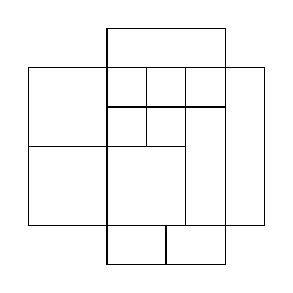
\begin{tikzpicture}[scale=.5]
      \draw(0,1)rectangle(6,5);
      \draw(2,0)rectangle(5,6);
      \draw(0,3)--(4,3)
           (3.5,0)--(3.5,1)
           (4,1)--(4,5)
           (2,4)--(5,4)
           (3,3)--(3,5);
    \end{tikzpicture}
  \end{center}
\end{example}
\begin{proof}[提示]首先最小的由单个四边形组成的共有13个。
  \begin{center}
    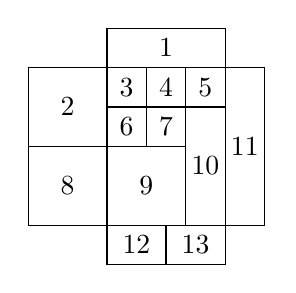
\begin{tikzpicture}[scale=.5]
      \draw(0,1)rectangle(6,5);
      \draw(2,0)rectangle(5,6);
      \draw(0,3)--(4,3)
           (3.5,0)--(3.5,1)
           (4,1)--(4,5)
           (2,4)--(5,4)
           (3,3)--(3,5);
           \foreach \n/\x/\y in{%
             1/3.5/5.5, 2/1/4, 3/2.5/4.5, 4/3.5/4.5, 5/4.5/4.5, 6/2.5/3.5, 7/3.5/3.5,
             8/1/2, 9/3/2, 10/4.5/2.5, 11/5.5/3, 12/2.75/.5, 13/4.25/.5}{%
             \node at(\x,\y){\n};
           }
    \end{tikzpicture}
  \end{center}

  由两个小四边形组成的共有9个:
  \begin{center}
    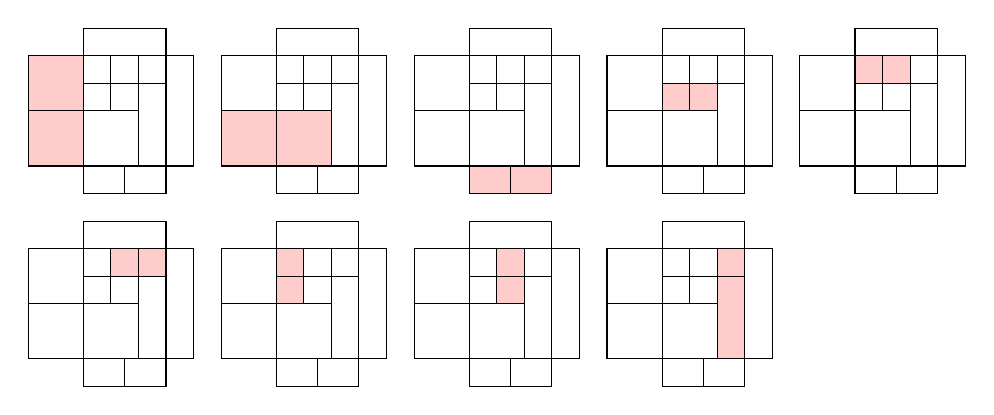
\begin{tikzpicture}[scale=.35]
      \foreach \dx/\dy/\x/\y/\xx/\yy in {%
        0/0/0/1/2/5, 7/0/0/1/4/3, 14/0/2/0/5/1, 21/0/2/3/4/4, 28/0/2/4/4/5, 
        0/7/3/4/5/5, 7/7/2/3/3/5, 14/7/3/3/4/5, 21/7/4/1/5/5
      }{
        \begin{scope}[shift={(\dx,-\dy)}]
          \fill[color=red!20](\x,\y)rectangle(\xx,\yy);
          \draw(0,1)rectangle(6,5);
          \draw(2,0)rectangle(5,6);
          \draw(0,3)--(4,3) (3.5,0)--(3.5,1) (4,1)--(4,5) (2,4)--(5,4) (3,3)--(3,5);
        \end{scope}
      }
    \end{tikzpicture}    
  \end{center}

  由三个小四边形组成的共有4个:
  \begin{center}
    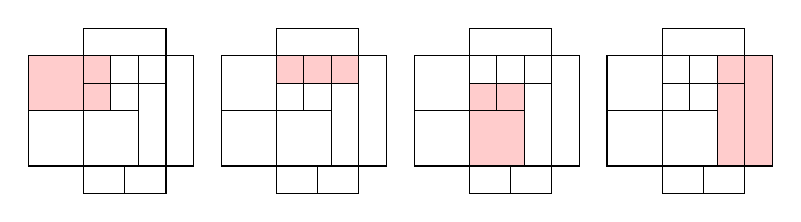
\begin{tikzpicture}[scale=.35]
      \foreach \dx/\dy/\x/\y/\xx/\yy in {%
        0/0/0/3/3/5, 7/0/2/4/5/5, 14/0/2/1/4/4, 21/0/4/1/6/5
      }{
        \begin{scope}[shift={(\dx,-\dy)}]
          \fill[color=red!20](\x,\y)rectangle(\xx,\yy);
          \draw(0,1)rectangle(6,5);
          \draw(2,0)rectangle(5,6);
          \draw(0,3)--(4,3) (3.5,0)--(3.5,1) (4,1)--(4,5) (2,4)--(5,4) (3,3)--(3,5);
        \end{scope}
      }
    \end{tikzpicture}    
  \end{center}
  
  由四个小四边形组成的共有3个:
  \begin{center}
    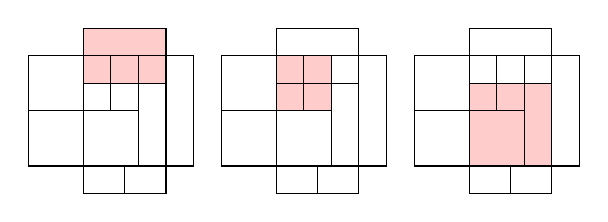
\begin{tikzpicture}[scale=.35]
      \foreach \dx/\dy/\x/\y/\xx/\yy in {%
        0/0/2/4/5/6, 7/0/2/3/4/5, 14/0/2/1/5/4
      }{
        \begin{scope}[shift={(\dx,-\dy)}]
          \fill[color=red!20](\x,\y)rectangle(\xx,\yy);
          \draw(0,1)rectangle(6,5);
          \draw(2,0)rectangle(5,6);
          \draw(0,3)--(4,3) (3.5,0)--(3.5,1) (4,1)--(4,5) (2,4)--(5,4) (3,3)--(3,5);
        \end{scope}
      }
    \end{tikzpicture}    
  \end{center}

  其余的自行考虑。
\end{proof}